%%%% PROCESAR con PdfLaTeX !!!!!


\documentclass[14pt]{book}
\usepackage[T1]{fontenc}
\usepackage{lmodern}
\usepackage{geometry}\geometry{top=2cm,bottom=2cm,left=2cm,right=2cm}
\usepackage{amssymb}
\usepackage{amsmath}
\usepackage{graphicx}
%\usepackage{txfonts}
%\usepackage{hyperref}
\usepackage[hidelinks]{hyperref}
\usepackage[spanish]{babel}
\setcounter{tocdepth}{4}
\usepackage[usenames]{color}
\usepackage{pdfpages}
\usepackage{enumerate}
\usepackage{framed}
\usepackage{color}
\usepackage{wrapfig}\definecolor{shadecolor}{RGB}{224,238,238}


\usepackage{multirow, array} % para las tablas
\usepackage{float} % para usar [H]




\usepackage[hidelinks]{hyperref}
\hypersetup{
    colorlinks=true,
    linkcolor=blue,
    filecolor=magenta,      
    urlcolor=cyan,
    pdftitle={Sharelatex Example},
    bookmarks=true,
%    pdfpagemode=FullScreen,
}



\begin{document}
\thispagestyle{empty}

\begin {center}


\includegraphics[scale=.4]{./img/logo.jpeg}


\medskip
\textbf{\large UNIVERSIDAD DE BUENOS AIRES}

Facultad de Ciencias Económicas \\
Departamento de Economía

\vspace{3cm}



\textbf{\large ESTADISTICA I}

\vspace{2cm}


Este es un modesto aporte para los alumnos de la f\'acultad de Econom\'ia  de la UBA.
De ninguna man\'era pretende ser una gu\'ia de estudio, ni remplaza las clases presenciales, el material oficial de la catedra esta disponible en el web site de la m\'ateria.
\\
\end {center}


\vspace{2.5cm}

\noindent Autor:	\,Isaac Edgar Camacho Ocampo
 
\noindent Carrera:	\,Licenciatura en Economía


\vspace{1cm}

\vspace{1cm}

\noindent Buenos Aires, 2021
\vspace{1cm}
\\
\textit{Si se encuentra alg\'un error u omisi\'on en este res\'umen por favor colaborar en  \\
\url{https://github.com/IsaacEdgarCamacho/Apuntes/} \quad \\ o escribirme a 
\url{isaac.edgar.camacho@gmail.com}
}
\newpage


\tableofcontents



\chapter{Combinatoria}

\section{Cardinal de conjuntos y cantidad de relaciones.:} La combinatoria es el arte de contar (en el sentido de enumerar, no de contar un cuento).  	\\

\subsection{Cardinal de un conjunto.}
Sea A un conjunto, se llama cardinal de A a la cantidad de elementos
distintos que tiene A , y se nota $\#A$ . Cuando el conjunto no tiene un
número finito de elementos, se dice que es infinito, y se nota $\#A = \infty$ . \\
 	Sean $A = \{a, b, c\}$ y $B = \{1, 2\} \Rightarrow \#A = 3, \#B = 2$ .
\subsection{Cardinal de un subconjunto.}
Sea A es un conjunto finito y sea $B \subseteq A$ . Entonces $\#B \leq \#A$ . \\
 	Sean $A = \{a, b, c\}$ y $B = \{c\} \Rightarrow \#A = 3, \#B = 1$ .
\subsection{Cardinal de la unión y del complemento}Sean A, B conjuntos finitos dentro de un conjunto referencial U . \\ 
 	Sean $A = \{a, b, c\}$ , $B = \{c,d,e \rbrace$ y $C = \{f\} \Rightarrow \#A = 3, \#B = 3,\#C = 1$ .
\begin{enumerate}[a)]
	\item Si A y B son conjuntos disjuntos, entonces $\#(A \cup B) = \#A + \#B$ . \\
		Ej.	$ \#(A \cup C) = 3+1=4 $
	\item En general $ \#(A \cup B) = \#A + \#B - \#(A \cap B)$. \\
			Ej.	$   \#(A \cup B) = 3 + 3 - 1 = 5. $		
	\item Si U es un conjunto finito, entonces $\#(A_c ) = \#U - \#A $.
\end{enumerate}


\subsection{Cardinal de un producto cartesiano y del conjunto de partes.}
Veamos ahora en un ejemplo como se comporta el cardinal del producto
cartesiano y del conjunto de partes. Sean $ A = \{a, b, c\}$ y $B = \{1, 2\} $ .
\subsubsection{Producto Cartesiano}
Sean A y B conjuntos finitos. Entonces $ \#(A \times B) = \#A \cdot \#B $ .\\
Esta es la famosa regla del producto, $ (A \times B) = \{(a,1),(b,1),(c,1),(a,2),(b,2),(c,2) \}$ y su cardinal es $ \#(A \times B) = 3\cdot 2 = 6$
\subsubsection{Conjunto Partes}


\subsection{Cantidad de relaciones y de funciones.}




%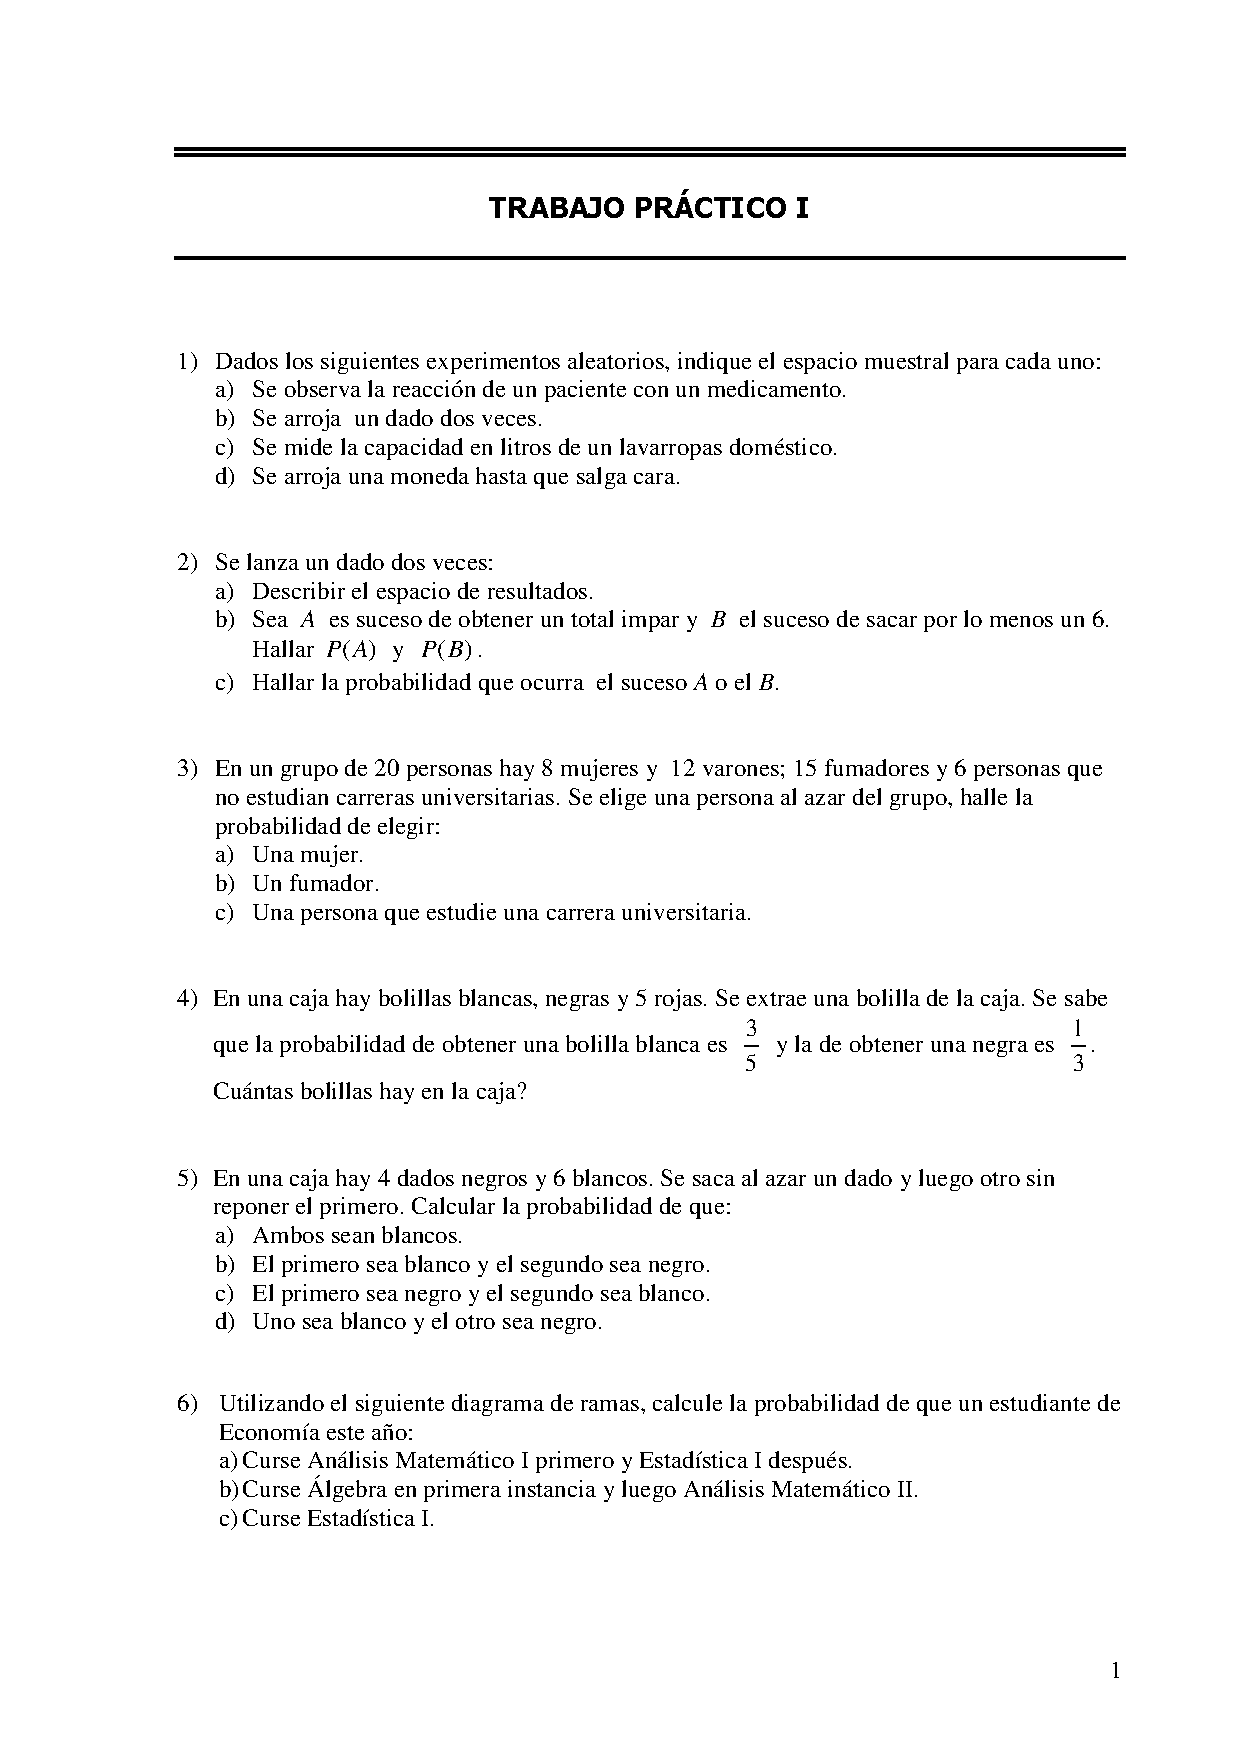
\includepdf[pages=-]{./pdfs/p1.pdf}

%\begin{center}
%    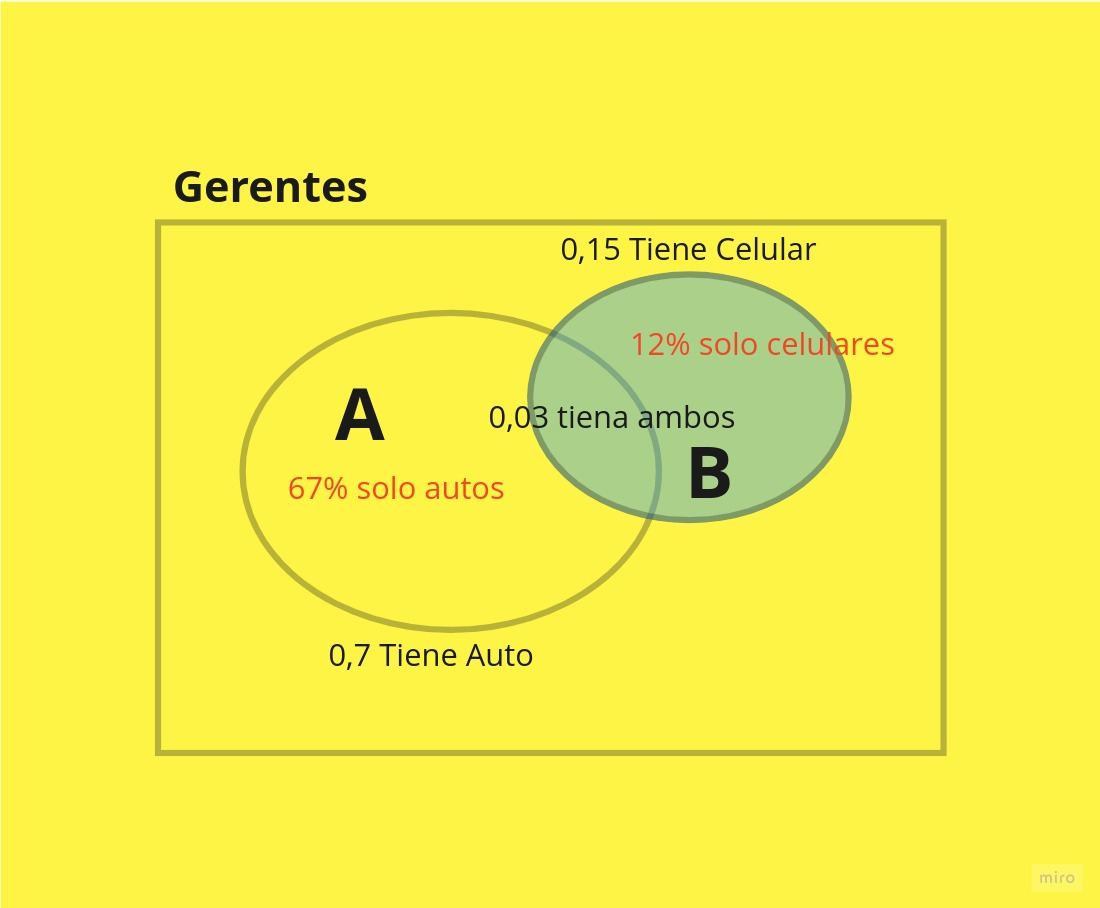
\includegraphics[scale=.2]{./img/ej11.jpg}    
%\end{center}

\end{document}


